\documentclass[12pt, a4paper]{article}

\usepackage[top=1.5cm, left=1.5cm, bottom=1.5cm, right=1.5cm]{geometry}
\usepackage{graphicx}

\usepackage[utf8]{inputenc}
\usepackage[T1]{fontenc}
\usepackage[francais]{babel}


\title{Rapport du jeu d'infection}
\author{CASTEL Flavien \and VOISIN Dan}
\date{02 Mars 2018}


\begin{document}
    
    \begin{titlepage}
        \begin{minipage}{0.4\linewidth}
            
\includegraphics{img/logo.png}
        \end{minipage}
        \hfill
        \begin{minipage}{0.4\linewidth}
            \begin{flushright}
                2017-2018
            \end{flushright}
        \end{minipage}
        
        \vspace{7cm}
        
        \begin{center}
            \textbf{\Huge{Rapport d'expérimentation du jeu d'infection}}
        \end{center}
        
        \vspace{9cm}
        
        \begin{minipage}{0.4\linewidth}
            CASTEL Flavien\\
            VOISIN Dan
        \end{minipage}
        \hfill
        \begin{minipage}{0.4\linewidth}
            \begin{flushright}
                L2 Informatique
            \end{flushright}
        \end{minipage}
        
    \end{titlepage}
    
    
    \section{Expérimentations sur la profondeur de recherche}
        Pour cette partie d'expérimentation, nous allons utiliser le même réseau ainsi que la même première machine infectée pour générer l'état initial. Celui-ci ressemble à la figure suivante:
        
        \begin{figure}[h]
            \centering
            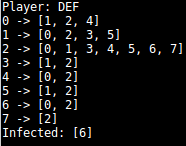
\includegraphics[scale=0.5]{img/state_init.png}
            \caption{État initial}
            \label{fig1}
        \end{figure}
        
        Nous renseignons le nombre de noeuds parcourus en fonction de la profondeur de recherche dans un fichier .dat afin de générer avec gnuplot le graphique suivant:
        
        \begin{figure}[h]
            \centering
            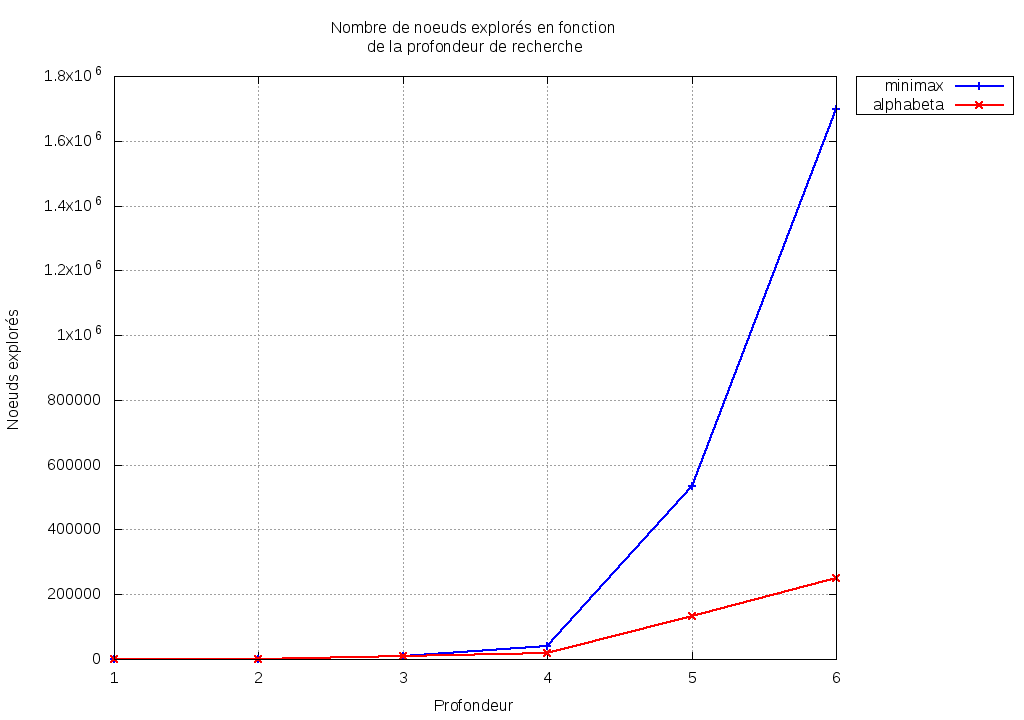
\includegraphics[scale=0.6]{img/graph1.png}
            \caption{Graphe comparant l'efficacité des deux algorithmes sur la profondeur}
            \label{fig2}
        \end{figure}
        
        Nous remarquons que les algorithmes parcourent les noeuds de manière exponentielle. De plus l'algorithme alphabeta devient véritablement efficace à partir d'une profondeur de quatre.
        
    \newpage
    \section{Expérimentation sur la probabilité}
        Pour l'expérimentation suivante, nous avons cumulé plusieurs test des algorithmes en utilisant une profondeur de recherche de quatre, d'un réseau composé de huit machines dont une seule est infectée aléatoirement. Puis nous faisons la moyenne du nombre de noeuds parcourus afin d'obtenir le graphique suivant:
        
        \begin{figure}[h]
            \centering
            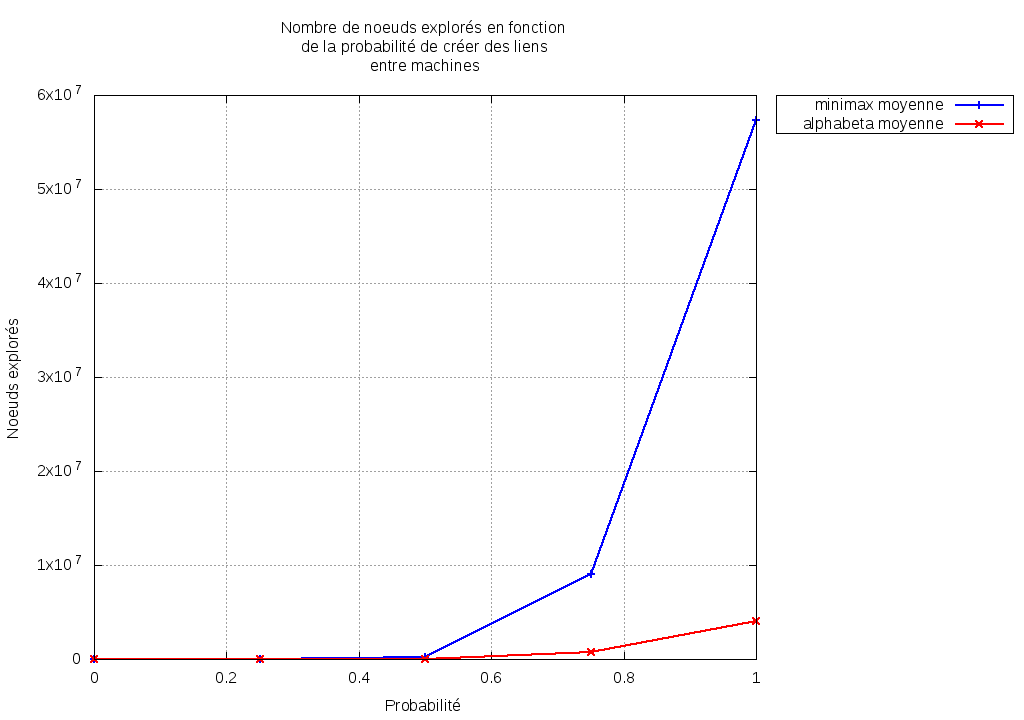
\includegraphics[scale=0.6]{img/graph2.png}
            \caption{Graphe comparant l'efficacité des deux algorithmes sur la probabilité}
            \label{fig3}
        \end{figure}
        
        Ici, nous nous apercevons que les deux algorithmes parcourent aussi de manière exponentielle les noeuds. De plus l'algorithme alphabeta devient plus efficace au delà d'une probabilité de 0.5.
        
\end{document}